\documentclass[12pt,letterpaper]{article}
\usepackage{graphicx,textcomp}
\usepackage{natbib}
\usepackage{setspace}
\usepackage{fullpage}
\usepackage{color}
\usepackage[reqno]{amsmath}
\usepackage{amsthm}
\usepackage{fancyvrb}
\usepackage{amssymb,enumerate}
\usepackage[all]{xy}
\usepackage{endnotes}
\usepackage{lscape}
\newtheorem{com}{Comment}
\usepackage{float}
\usepackage{hyperref}
\newtheorem{lem} {Lemma}
\newtheorem{prop}{Proposition}
\newtheorem{thm}{Theorem}
\newtheorem{defn}{Definition}
\newtheorem{cor}{Corollary}
\newtheorem{obs}{Observation}
\usepackage[compact]{titlesec}
\usepackage{dcolumn}
\usepackage{tikz}
\usetikzlibrary{arrows}
\usepackage{multirow}
\usepackage{xcolor}
\newcolumntype{.}{D{.}{.}{-1}}
\newcolumntype{d}[1]{D{.}{.}{#1}}
\definecolor{light-gray}{gray}{0.65}
\usepackage{url}
\usepackage{listings}
\usepackage{color}
\usepackage{indentfirst}

\definecolor{codegreen}{rgb}{0,0.6,0}
\definecolor{codegray}{rgb}{0.5,0.5,0.5}
\definecolor{codepurple}{rgb}{0.58,0,0.82}
\definecolor{backcolour}{rgb}{0.95,0.95,0.92}

\lstdefinestyle{mystyle}{
	backgroundcolor=\color{backcolour},   
	commentstyle=\color{codegreen},
	keywordstyle=\color{magenta},
	numberstyle=\tiny\color{codegray},
	stringstyle=\color{codepurple},
	basicstyle=\ttfamily\footnotesize,
	breakatwhitespace=false,         
	breaklines=true,                 
	captionpos=b,                    
	keepspaces=true,                 
	numbers=left,                    
	numbersep=5pt,                  
	showspaces=false,                
	showstringspaces=false,
	showtabs=false,                  
	tabsize=2
}
\lstset{style=mystyle}
\newcommand{\Sref}[1]{Section~\ref{#1}}
\newtheorem{hyp}{Hypothesis}
\renewcommand{\contentsname}{Table of Contents}
	
\title{Final Project: U.S. Border Crossing Entries}
\date{Due: March 9, 2026}
\author{Data Visualization\\
	Shelly Veal-Upham\\
	25337422}
	
\begin{document}
	\maketitle
	\tableofcontents
		
	
	\section*{Executive Summary}
	\addcontentsline{toc}{section}{Executive Summary}
	
	 These pages comprise my final project for Data Visualization in Spring 2026. I will walk you through three main visualizations I chose to represent the dataset of my choosing, "Border Crossing Entry Data." These figures are meant both as practice for me in the use of \texttt{R} for data visualization and as tools for answering basic questions relating to the movement of people into the United States over time. Because I am using only one dataset and will not reference other specific data sources for the corroboration of any claims, I will make no causal inferences about what trends I may identify in the data, but will suggest theories and potential further inquiries to be made in explaining the data. \\
	 
	 First I will clarify the tools I used in R and the background of my dataset. Next, I will share the overall data manipulation steps I took prior to the creation of my plots. Finally, for each of my figures, I will explain their intended purpose the process of their creation in \texttt{R} before sharing the plots themselves. \\
	 
	 I used the following packages in R: \\
	 
	 	\lstinputlisting[language = R, firstline=26, lastline=29]{final_project.r} 
	 	
	I also utilized my custom theme for the graphics, relying on \texttt{showtext}, \texttt{systemfonts}, and \texttt{purrr} for its proper rendering on my device: \\
	
	\lstinputlisting[language = R, firstline=50, lastline=73]{final_project.r} 
	
	\section*{Data Background}
	\addcontentsline{toc}{section}{Data Background}
	 The dataset in use for this project comprises border crossing entry data collected by the Bureau of Transportation Statistics in the United States (U.S.) and posted publicly on Kaggle at:\\
	 
	 {https://www.kaggle.com/datasets/akhilv11/border-crossing-entry-data} \\
	  
	 The dataset only reports those \textbf{entering} the U.S., and not those \textbf{exiting} the U.S. Henceforth any use of the term "crossing" will refer to those crossing the border to \textbf{enter} the U.S. The unit of observation in the dataset is a monthly aggregate of vehicles (by various type - train, bus, etc.) or persons (by nature of individual crossing - pedestrian, personal vehicle, etc.) crossing the border at each port ranging from 1996 to 2019.\\
	
	 
	\section*{Data Cleaning}
	\addcontentsline{toc}{section}{Data Cleaning}
	In the line of data cleaning, I had little to do except complete a few formatting adjustments such that the \texttt{Location} column was split into separate \texttt{Latitude} and \texttt{Longitude} columns for ease of my initial visualizations (although this would later be undone during the simple features transormation using package \texttt{usmap}). I also dropped "Calexico East" data (Port code: 2507) given the note in the codebook that "Calexico" already includes "Calexico East" numbers. 
	
	\lstinputlisting[language = R, firstline=95, lastline=104]{final_project.r}
	
	Because my interest lies in people crossing the border (rather than commercial transportation of goods as captured by the vehicle crossing data in this dataset), I first reduced my dataset to comprise only of individuals recorded entering the U.S.\\
	
	\lstinputlisting[language = R, firstline=108, lastline=111]{final_project.r}


	\section*{Individual Figures}
	\addcontentsline{toc}{section}{Individual Figures}

	\subsection*{Fig 1: Geography of Crossings}
		\addcontentsline{toc}{subsection}{Fig 1: Geography of Crossings}
		
		Taking a look at the geographical dispersion of our ports of entry provides a broad overview of the main story of our data-- where do people enter the U.S. the most, on average? Are there a higher concentration of entry ports in certain areas than others?\\
			
		To create Figure~\ref{fig1}, I ensured my data was compiled geographically such that the average number of people crossing each year would display nicely on a figure that includes Alaska (provided by the package \texttt{usmap}).
			
			\lstinputlisting[language = R, firstline=124, lastline=139]{final_project.r}
			
			Using the package \texttt{usmap}, I plotted the data:
			
			\lstinputlisting[language = R, firstline=141, lastline=154]{final_project.r}
			
	\begin{figure}[h!]
		\caption{Average Yearly Crossings Map}\label{fig1}
		\centering
		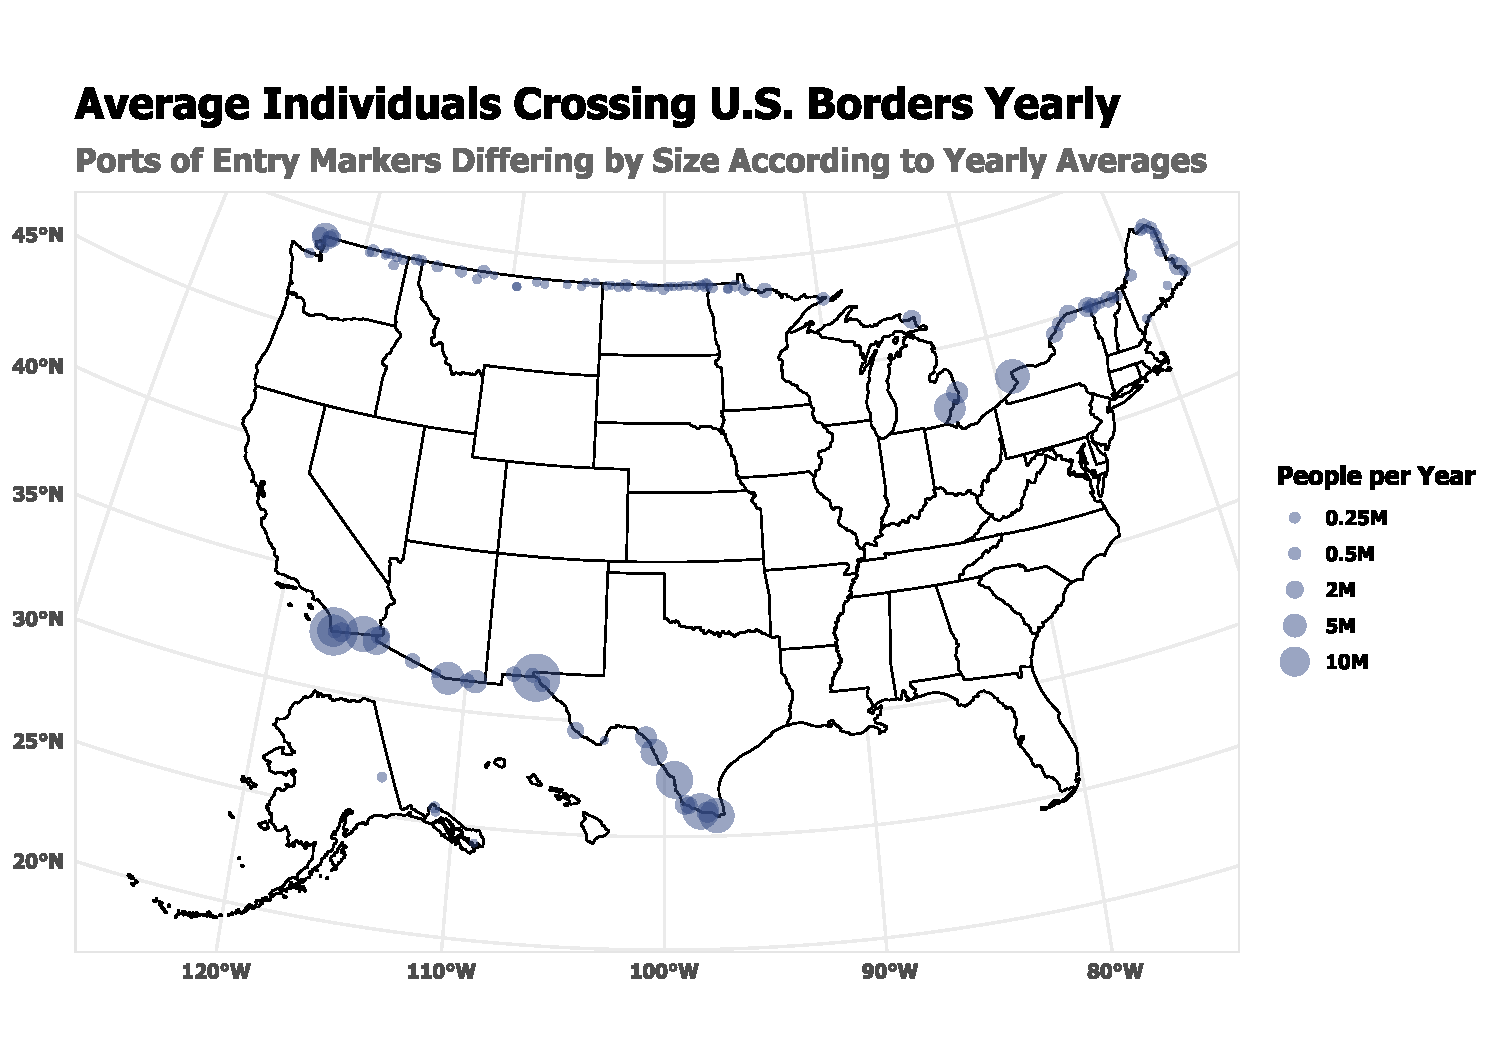
\includegraphics[width=1\textwidth]{individual_figures/map.pdf}
	\end{figure}
	
	 Upon visualization, we can see that California and Texas take on the most crossings in the south, while Michigan and New York appear to accept the largest number of entrants in the north. Still, this map relies solely on yearly averages of people entering the U.S. at each port. For a more nuanced understanding of the data, we will need to dig deeper in further visualizations. 
	 
	\newpage
	\subsection*{Fig 2: State Differences}
		\addcontentsline{toc}{subsection}{Fig 2: State Differences}
		
	The boxplots below display the distribution of yearly border crossings per state between 1996 and 2019.  Figure~\ref{fig2} shows states with US-Canada borders while Figure~\ref{fig3} consists of states with US-Mexico borders. \\
	
	For plotting, I first created the main dataframe by aggregating yearly crossings by state and dividing by one million such that my unit of observation was millions of people:
	
	\lstinputlisting[language = R, firstline=163, lastline=168]{final_project.r}
	
	I then created the plots for US-Mexico and US-Canada borders respectively:
	
	\lstinputlisting[language = R, firstline=171, lastline=191]{final_project.r}

\begin{figure}[h!]
	\caption{Yearly Crossings per State, US-Canada Border}\label{fig2}
	\centering
	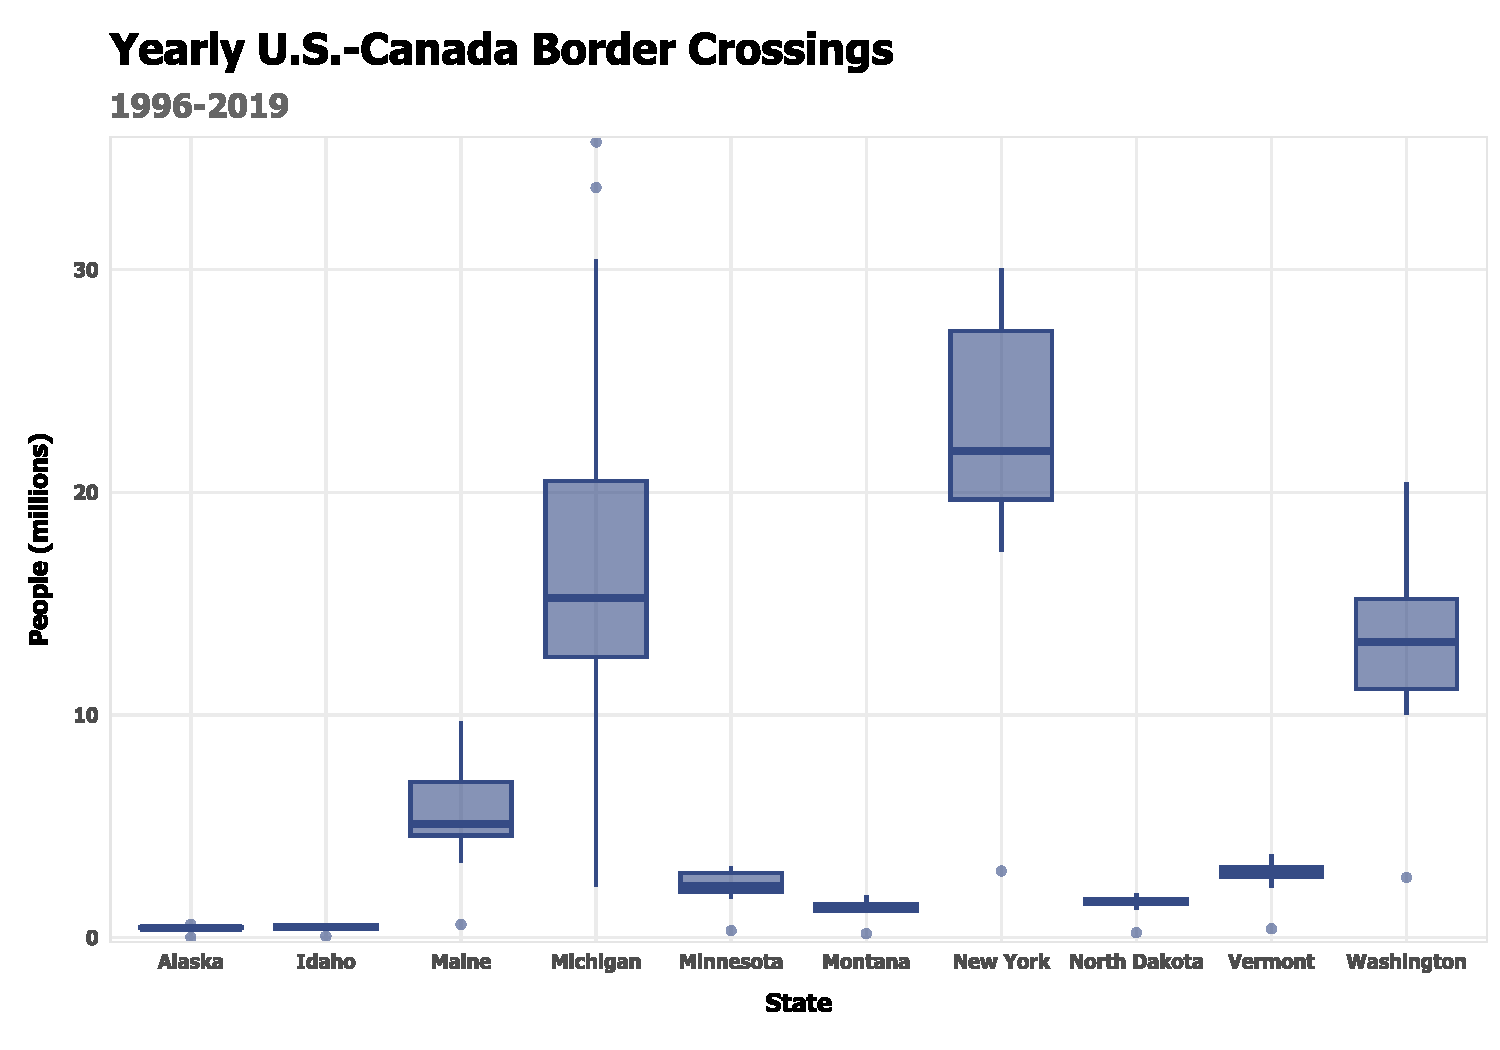
\includegraphics[width=.8\textwidth]{individual_figures/ca_bp.pdf}
\end{figure}

\begin{figure}[h!]
	\caption{Yearly Crossings per State, US-Mexico Border}\label{fig3}
	\centering
	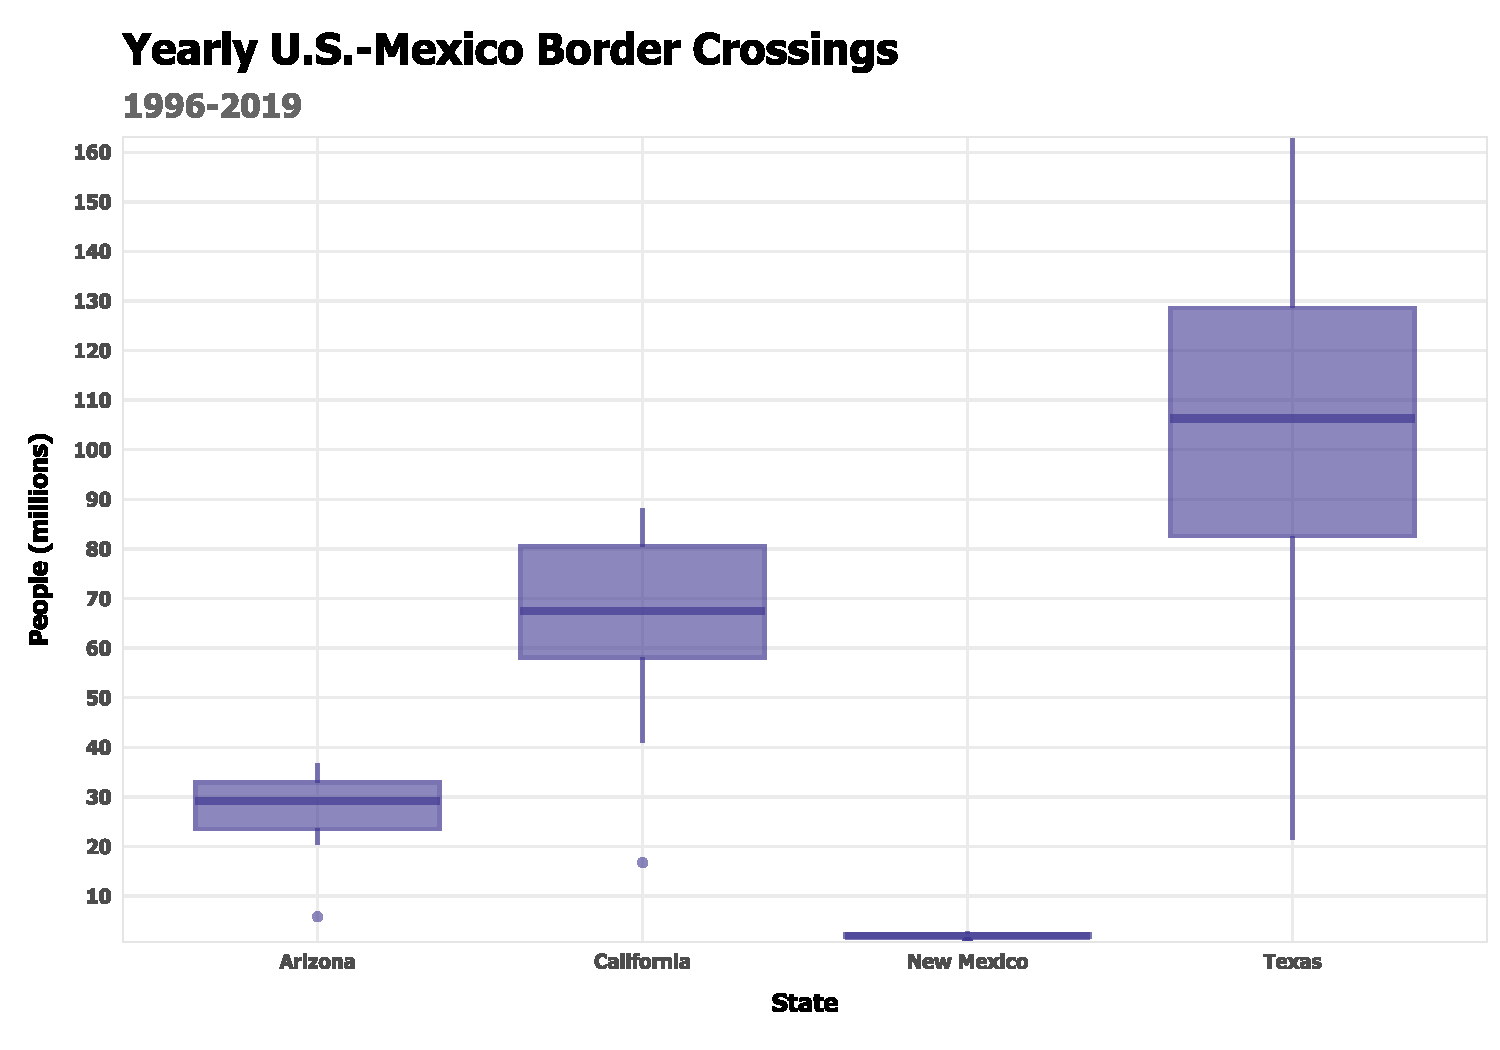
\includegraphics[width=.8\textwidth]{individual_figures/mx_bp.pdf}
\end{figure}
\newpage

	The first striking component of these figures is the difference between the scales-- Texas and California's average yearly crossings stretch the US-Mexico graph scales from 0 all the way to 160 million people, while the US-Canada crossings graph is caputered within the range of 0-40 million. One might utilize this data in conjunction with other state-specific information to build an understanding of the relationships U.S. states and their citizens have with their physical international borders (i.e. do a higher number of entrants to one's state correlate with particular positions on immigration or international trade policies?). Without this added context, it is still interesting to note the severe difference in port crossings among states. \\

\newpage
\subsection*{Fig 3: Trends Over Time}
		\addcontentsline{toc}{subsection}{Fig 3: Trends Over Time}
		
	Finally, it is informative to investigate changes in entries over time for each of the borders (see Figures ~\ref{fig4} \&~\ref{fig5}). By visualizing the total, trend, seasonality, and residual changes for each border, we can see that crossings of the U.S.-Canada border follow stricter seasonality than the U.S.-Mexico border, with more entries over summer months than winter ones, perhaps due to the operation of ferries in the summertime. We can also see that entries from Canada on the whole have decreased, whereas the lowest number of monthly entries from Mexico occurred in 2011, and have steadily risen overall since. These are only a few insights that could be gathered from the visualizations, created using the following process:\\
	
	 I first aggregated data by border and date (month):
	
	\lstinputlisting[language = R, firstline=195, lastline=197]{final_project.r}
	
	 Next, utilizing base package \texttt{stats}, I decomposed the time-series information for all of the data relating to each border in our time period (1996 - 2019). From this data, I derived dataframes for Canada and Mexico respectively, with splits for top and bottom charts. Separating the Seasonal/Residual changes from the Total and Trend graphs is essential, given the vast difference in their scales. I also created separate objects for the minimum and maximum individual crossings in a month's time, such that I could visualize the point in time at which there were the most and least overall entries to the U.S. at each border:\\
	 
	Canada:
	
	\lstinputlisting[language = R, firstline=210, lastline=253]{final_project.r}
	
	Mexico:
	
	\lstinputlisting[language = R, firstline=301, lastline=337]{final_project.r}
	
	Then I plotted both top and bottom components and stacked them using the package \texttt{patchwork}.\\
	
	Canada:
	\lstinputlisting[language = R, firstline=257, lastline=295]{final_project.r}
	
	Mexico:
	\lstinputlisting[language = R, firstline=341, lastline=379]{final_project.r}
\newpage

\begin{figure}[h!]
	\caption{US-Canada Crossings Trends Over Time}\label{fig4}
	\centering
	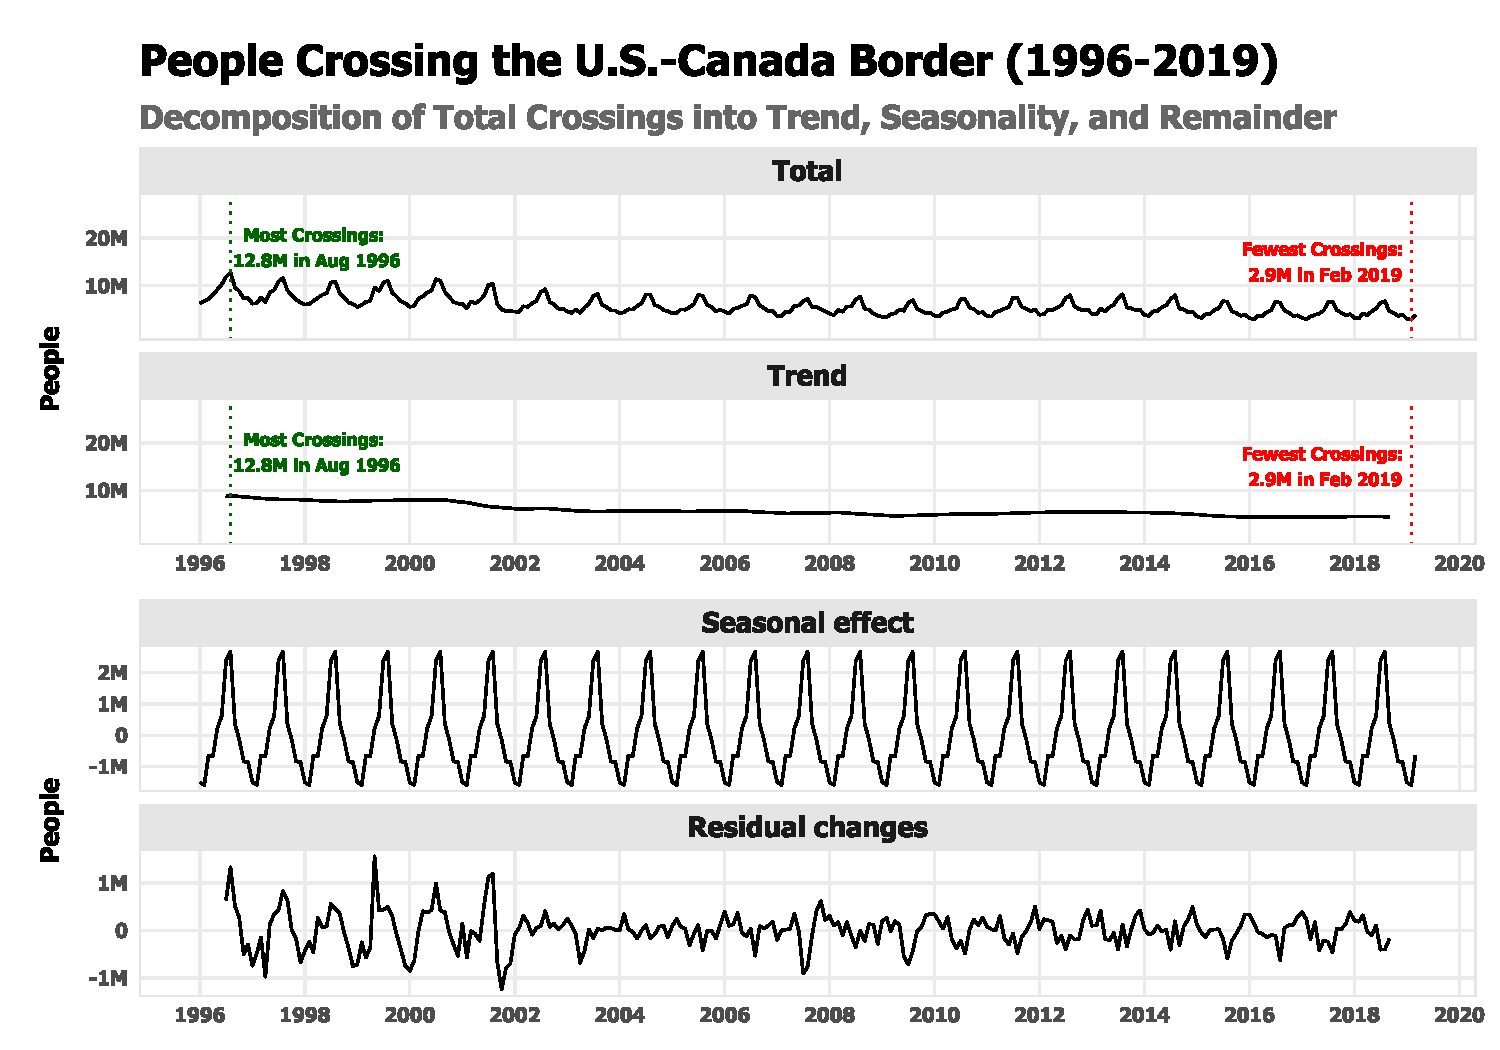
\includegraphics[width=.81\textwidth]{individual_figures/ca_timescale.pdf}
\end{figure}
\vspace{-0.7cm}
\begin{figure}[h!]
	\caption{US-Mexico Crossings Trends Over Time}\label{fig5}
	\centering
	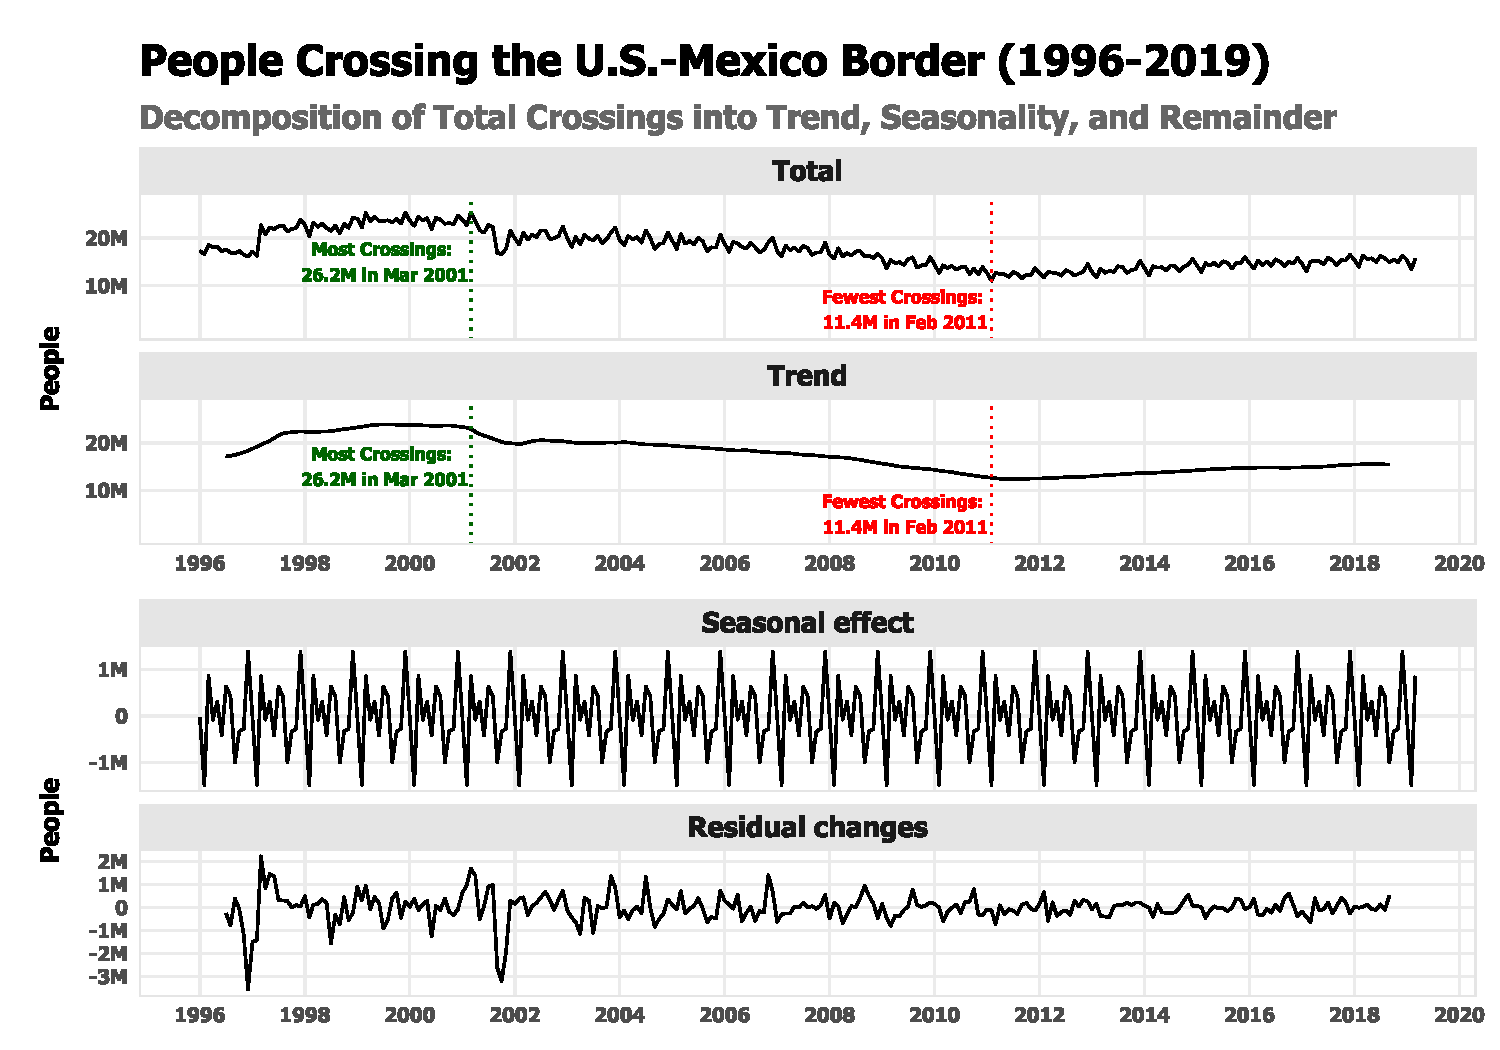
\includegraphics[width=.81\textwidth]{individual_figures/mx_timescale.pdf}
\end{figure}

\end{document}
